% !TEX program = xelatex
\documentclass[a4paper]{exam}
\usepackage{amsmath}
\usepackage{amsthm}
\usepackage[left=1.8cm,right=1.8cm,top=2.2cm,bottom=2.0cm]{geometry}
\usepackage[UTF8]{ctex}
\usepackage{enumerate}
\usepackage{fancyhdr}
\usepackage{xpatch}
\usepackage{graphicx} 
\usepackage{float} 
\usepackage{subfigure} 
\usepackage{amsfonts}
\usepackage{mathtools}
\usepackage{framed}
\usepackage{multicol}
\usepackage{minted}
\usepackage{fontspec}
\usepackage{float}
\usepackage{tikz}
\usepackage{alltt}
\usepackage{multicol,comment}
\usepackage{biblatex}
\addbibresource{02-discussion.bib}
\usetikzlibrary{automata,positioning}
\usepackage[section]{placeins}
\makeatletter

\printanswers


\AtBeginDocument{\xpatchcmd{\@thm}{\thm@headpunct{.}}{\thm@headpunct{}}{}{}}
\makeatother

\pagestyle{fancy}
\renewcommand{\baselinestretch}{1.15}
\newcommand{\code}[1]{\texttt{#1}}
\usepackage{paralist}
\let\itemize\compactitem
\let\enditemize\endcompactitem
\let\enumerate\compactenum
\let\endenumerate\endcompactenum
\let\description\compactdesc
\let\enddescription\endcompactdesc

% shorten footnote rule
\xpatchcmd\footnoterule
  {.4\columnwidth}
  {1in}
  {}{\fail}

\title{CS 131 Compilers: Discussion 2: (Non)Deterministic Finite Automata \& Top-Down Parsers}
\author{\textbf{杨易为}~~\textbf{吴凌云}~~\textbf{樊雨鑫} \\ \texttt{ \{yangyw,wuly2,fanyx\}@shanghaitech.edu.cn}}

\begin{document}
\maketitle
\section{DFA and NFA}
\subsection{Introduction}

Finite-state automata (FSA) are abstract machines that feature states and guarded transitions from one state to another. An FSA can only be in one state a time, and its total number of states is finite.  The machine takes transitions in response to inputs it receives sequentially;  if an input matches the guard of a transition that departs from the current state that transition is said to be enabled; only enabled transitions can be taken.  FSA that have an accepting state provide the machinery to determine whether an input string is in a regular language.  If no transitions are enabled by a given input then the entire input string gets  rejected.   If  all  inputs  are  processed  and  the  FSA  is  in  an  accepting  state  then  the entire input string is accepted.  Deterministic finite state automata (DFA) can only have one enabled transition at a time while a non-deterministic finite state automata (NFA) can have multiple.
\\
Before NLP, we utilize state machines to accept languages. Two different perspectives can be considered, namely symbolic and random. chomsky's formal language theory embodies a symbolic approach. Based on this view, a language contains a sequence of symbols that must follow the syntactic rules of its generative grammar. This view reduces the structure of a language to a set of well-defined rules that allow for the decomposition of each sentence and word into structural components.
\subsection{Examples of accepting x86 Assembly\cite{bcst}}
There are three main types of terminators for assembly instructions: Immediately and Scale for numbers, Reg and Op for characters, and other symbols, including spaces (' '), commas (','), and parentheses ('(',')'). For numeric terminators, we can use Deterministic Finite Automation (DFA) to determine and parse them according to Regular Grammar, see below Figure. It should be noted that the numbers in assembly instructions include positive and negative integers in hexadecimal and decimal, and We need to check whether the value overflows at each state transfer step.

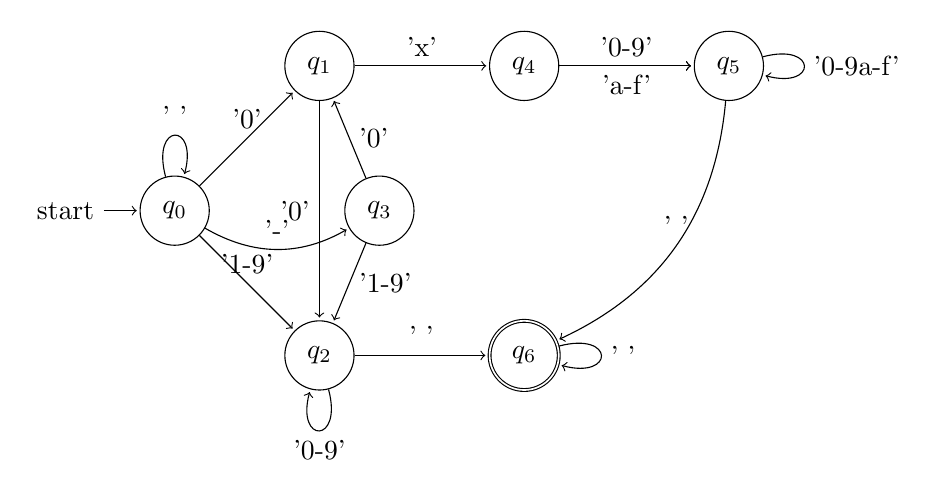
\begin{tikzpicture}[shorten >=1pt,node distance=2.6cm,on grid,auto]
    \node[state,initial] (q_0)   {$q_0$};
    \node[state] (q_1) [ above right=of q_0] {$q_1$};
    \node[state] (q_2) [below right=of q_0] {$q_2$};
    \node[state] (q_3) [ right=of q_0] {$q_3$};
    \node[state] (q_4) [ right=of q_1] {$q_4$};
    \node[state] (q_5) [ right=of q_4] {$q_5$};
    \node[state,accepting] (q_6) [ right=of q_2] {$q_6$};
    \path[->]
    (q_0) edge [loop above] node {' '} ()
    edge  node  [above]{'0'} (q_1)
    edge [bend right] node  [above]{'-'} (q_3)
    edge  node  [above]{'1-9'} (q_2)
    (q_1) edge  node  {'x'} (q_4)
    edge node [left] {'0'} (q_2)
    (q_2) edge  node  {' '} (q_6)
    edge [loop below] node {'0-9'} ()
    (q_3)edge  node [right] {'0'} (q_1)
    edge  node [right] {'1-9'} (q_2)
    (q_4)edge  node  {'0-9'} (q_5)
    edge [below] node  {'a-f'} (q_5)
    (q_5) edge [loop right] node {'0-9a-f'} ()
    edge [bend left] node [above] {' '} (q_6)
    (q_6) edge [loop right] node {' '} ()
    ;

\end{tikzpicture}\\
For character type terminators, i.e. operands and registers, we can take a simple string matching (Matching). Here, we have a variety of data structures to employ. The most common approach is to use an array or list that stores all possible string values, e.g., \{"rax","eax"\} and \{"mov","ld","sd"\}, and iterate through this array and match each element. With such a data structure, the time complexity of finding and matching is $O(LE[strlen])$, where $E[strlen]$ is the average length of the string. Another strategy is to build a dictionary tree (Trie) or a prefix tree for the above array of strings.
\\
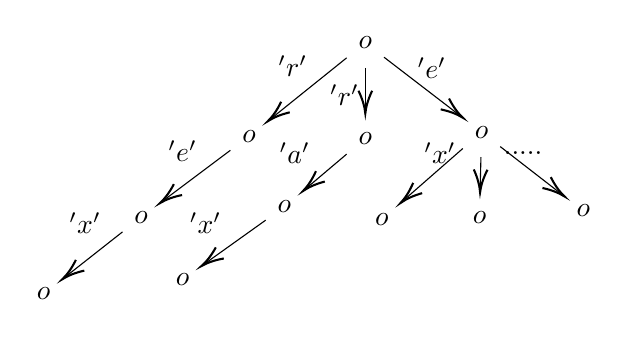
\begin{tikzpicture}[x=0.75pt,y=0.75pt,yscale=-1,xscale=1]
    %uncomment if require: \path (0,235); %set diagram left start at 0, and has height of 235


    % Text Node
    \draw (154,44) node    {$o$};
    % Text Node
    \draw (98,89) node    {$o$};
    % Text Node
    \draw (119,55) node    {$'r'$};
    % Text Node
    \draw (154,90) node    {$o$};
    % Text Node
    \draw (210,87) node    {$o$};
    % Text Node
    \draw (144,69) node    {$'r'$};
    % Text Node
    \draw (186,56) node    {$'e'$};
    % Text Node
    \draw (66,96) node    {$'e'$};
    % Text Node
    \draw (46,128) node    {$o$};
    % Text Node
    \draw (-1,165) node    {$o$};
    % Text Node
    \draw (19,131) node    {$'x'$};
    \draw (77,131) node    {$'x'$};
    % Text Node
    \draw (115,123) node    {$o$};
    % Text Node
    \draw (120,97) node    {$'a'$};
    \draw (190,97) node    {$'x'$};
    \draw (230,97) node    {$.....$};
    % Text Node
    \draw (66,158) node    {$o$};
    % Text Node
    \draw (162,129) node    {$o$};
    % Text Node
    \draw (209,128) node    {$o$};
    % Text Node
    \draw (259,125) node    {$o$};
    % Connection
    \draw    (145,51.23) -- (108.56,80.52) ;
    \draw [shift={(107,81.77)}, rotate = 321.22] [color={rgb, 255:red, 0; green, 0; blue, 0 }  ][line width=0.75]    (10.93,-3.29) .. controls (6.95,-1.4) and (3.31,-0.3) .. (0,0) .. controls (3.31,0.3) and (6.95,1.4) .. (10.93,3.29)   ;
    % Connection
    \draw    (154,56) -- (154,76) ;
    \draw [shift={(154,78)}, rotate = 270] [color={rgb, 255:red, 0; green, 0; blue, 0 }  ][line width=0.75]    (10.93,-3.29) .. controls (6.95,-1.4) and (3.31,-0.3) .. (0,0) .. controls (3.31,0.3) and (6.95,1.4) .. (10.93,3.29)   ;
    % Connection
    \draw    (163,50.91) -- (199.41,78.87) ;
    \draw [shift={(201,80.09)}, rotate = 217.52] [color={rgb, 255:red, 0; green, 0; blue, 0 }  ][line width=0.75]    (10.93,-3.29) .. controls (6.95,-1.4) and (3.31,-0.3) .. (0,0) .. controls (3.31,0.3) and (6.95,1.4) .. (10.93,3.29)   ;
    % Connection
    \draw    (89,95.75) -- (56.6,120.05) ;
    \draw [shift={(55,121.25)}, rotate = 323.13] [color={rgb, 255:red, 0; green, 0; blue, 0 }  ][line width=0.75]    (10.93,-3.29) .. controls (6.95,-1.4) and (3.31,-0.3) .. (0,0) .. controls (3.31,0.3) and (6.95,1.4) .. (10.93,3.29)   ;
    % Connection
    \draw    (37,135.09) -- (9.57,156.68) ;
    \draw [shift={(8,157.91)}, rotate = 321.78999999999996] [color={rgb, 255:red, 0; green, 0; blue, 0 }  ][line width=0.75]    (10.93,-3.29) .. controls (6.95,-1.4) and (3.31,-0.3) .. (0,0) .. controls (3.31,0.3) and (6.95,1.4) .. (10.93,3.29)   ;
    % Connection
    \draw    (145,97.62) -- (125.53,114.09) ;
    \draw [shift={(124,115.38)}, rotate = 319.76] [color={rgb, 255:red, 0; green, 0; blue, 0 }  ][line width=0.75]    (10.93,-3.29) .. controls (6.95,-1.4) and (3.31,-0.3) .. (0,0) .. controls (3.31,0.3) and (6.95,1.4) .. (10.93,3.29)   ;
    % Connection
    \draw    (106,129.43) -- (76.63,150.41) ;
    \draw [shift={(75,151.57)}, rotate = 324.46000000000004] [color={rgb, 255:red, 0; green, 0; blue, 0 }  ][line width=0.75]    (10.93,-3.29) .. controls (6.95,-1.4) and (3.31,-0.3) .. (0,0) .. controls (3.31,0.3) and (6.95,1.4) .. (10.93,3.29)   ;
    % Connection
    \draw    (201,94.88) -- (172.51,119.81) ;
    \draw [shift={(171,121.13)}, rotate = 318.81] [color={rgb, 255:red, 0; green, 0; blue, 0 }  ][line width=0.75]    (10.93,-3.29) .. controls (6.95,-1.4) and (3.31,-0.3) .. (0,0) .. controls (3.31,0.3) and (6.95,1.4) .. (10.93,3.29)   ;
    % Connection
    \draw    (209.71,99) -- (209.34,114) ;
    \draw [shift={(209.29,116)}, rotate = 271.4] [color={rgb, 255:red, 0; green, 0; blue, 0 }  ][line width=0.75]    (10.93,-3.29) .. controls (6.95,-1.4) and (3.31,-0.3) .. (0,0) .. controls (3.31,0.3) and (6.95,1.4) .. (10.93,3.29)   ;
    % Connection
    \draw    (219,93.98) -- (248.42,116.79) ;
    \draw [shift={(250,118.02)}, rotate = 217.79] [color={rgb, 255:red, 0; green, 0; blue, 0 }  ][line width=0.75]    (10.93,-3.29) .. controls (6.95,-1.4) and (3.31,-0.3) .. (0,0) .. controls (3.31,0.3) and (6.95,1.4) .. (10.93,3.29)   ;

\end{tikzpicture}


By using prefix trees, searching and matching can be done without traversing the entire array, and the time complexity is reduced to $O(E[strlen])$. In the implementation, a prefix tree can be created for all instruction operator names and register names before executing the CPU instruction cycle, so that the matching time can be reduced during the execution of the instruction cycle. Each node of the prefix tree usually includes a char$\rightarrow$(void *) mapped data structure, where char is the character and (void *) is the address of the subtree. As you can see, the prefix tree is very similar to the DFA, except that the prefix tree automatically builds the state transfer (so it is not streamlined enough), while the DFA requires us to calculate the state transfer in advance.
\subsection{Examples of accepting yaml}
We cannot do it, because of indent can only be accepted with stack machine.

\begin{minted}[mathescape, linenos]{yaml}
// Identity definitions
<whitespace> ::= " " | "\t"
<in-line-whitespace> ::= <whitespace> | <whitespace> <in-line-whitespace>
<digit> ::= "0" | "1" | "2" | "3" | "4" | "5" | "6" | "7" | "8" | "9"
<integer-number> ::= <digit> | <digit> <integer-number>
<end-of-line> ::= "\r\n" | "\r" | "\n"
<non-whitespace> ::=
<non-whitespace-word> ::= <non-whitespace> | <non-whitespace> <non-whitespace-word>
// Basic document structure
<yaml-stream> ::= <yaml-document-list>
<yaml-document-list> ::= <yaml-document> | <yaml-document> <yaml-document-list>
<yaml-document> ::= <yaml-directive-list> <yaml-directives-end> <yaml-content-list>
        <yaml-document-end>
<yaml-directive-list> ::= <yaml-directive> <yaml-directive-list> | ""
<yaml-directive> ::= <yaml-directive-yaml> | <yaml-directive-tag>
<yaml-directive-yaml> ::= "%YAML" <in-line-whitespace> <integer-number> "." <integer-number>
         <end-of-line> | ""
<yaml-directive-tag> ::= "%TAG" <in-line-whitespace> <yaml-tag-handle> <in-line-whitespace> 
        <yaml-tag-prefix> <end-of-line> <yaml-directive-tag> | ""
<yaml-tag-handle> ::= "!" | "!!" | "!" <non-whitespace-word> "!"
<yaml-tag-prefix> ::= "!" <non-whitespace-word> | <non-whitespace-word>
<yaml-directives-end> ::= "---" | ""
<yaml-content-list> ::= <yaml-content> <yaml-content-list> | <yaml-content> <end-of-line>
<yaml-document-end> ::= "..." | ""
// Internals of an individual document
<yaml-content> ::= ...
\end{minted}

\subsection{What language is accepted by the following DFA?}
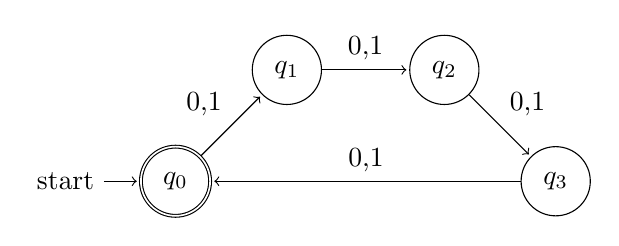
\begin{tikzpicture}[shorten >=1pt,node distance=2cm,on grid,auto]
    \node[state,initial,accepting] (q_0)   {$q_0$};
    \node[state] (q_1) [above right=of q_0] {$q_1$};
    \node[state] (q_2) [right=of q_1] {$q_2$};
    \node[state] (q_3) [below right=of q_2] {$q_3$};
    \path[->]
    (q_0) edge  node {0,1} (q_1)
    (q_1) edge  node  {0,1} (q_2)
    (q_2) edge  node  {0,1} (q_3)
    (q_3)edge  node  [above]{0,1} (q_0);

\end{tikzpicture}
\begin{solution}
    Binary strings of length 4 or multiples of 4, and the empty string.
\end{solution}

\subsection{What language is accepted by the following NFA?}
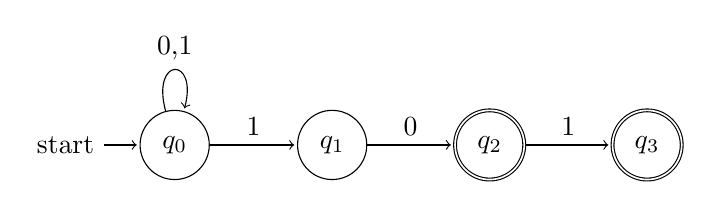
\begin{tikzpicture}[shorten >=1pt,node distance=2cm,on grid,auto]
    \node[state,initial] (q_0)   {$q_0$};
    \node[state] (q_1) [ right=of q_0] {$q_1$};
    \node[state,accepting] (q_2) [right=of q_1] {$q_2$};
    \node[state,accepting] (q_3) [ right=of q_2] {$q_3$};
    \path[->]
    (q_0) edge [loop above] node {0,1} ()
    edge  node  [above]{1} (q_1)
    (q_1) edge  node  {0} (q_2)
    (q_2) edge  node  {1} (q_3);

\end{tikzpicture}
\begin{solution}
    Binary strings ending in 10 or $101 .$
\end{solution}

\subsection{Construct a DFA that accepts binary strings of any length, except $3 .$}
\begin{solution}
    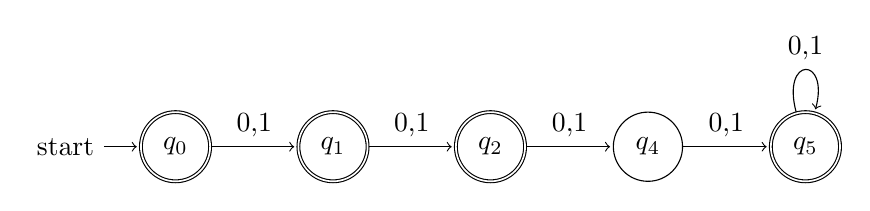
\begin{tikzpicture}[shorten >=1pt,node distance=2cm,on grid,auto]
        \node[state,initial,accepting] (q_0)   {$q_0$};
        \node[state,accepting] (q_1) [ right=of q_0] {$q_1$};
        \node[state,accepting] (q_2) [ right=of q_1] {$q_2$};
        \node[state] (q_3) [ right=of q_2] {$q_4$};
        \node[state,accepting] (q_4) [ right=of q_3] {$q_5$};
        \path[->]
        (q_0)
        edge  node  [above]{0,1} (q_1)
        (q_1) edge  node  {0,1} (q_2)
        (q_2) edge  node  {0,1} (q_3)
        (q_3) edge  node  {0,1} (q_4)
        (q_4) edge [loop above] node {0,1} ();
    \end{tikzpicture}
\end{solution}


\subsection{Construct the NFA that accepts}
\subsubsection{$x(zy?|(yz)*)$}
\begin{solution}
    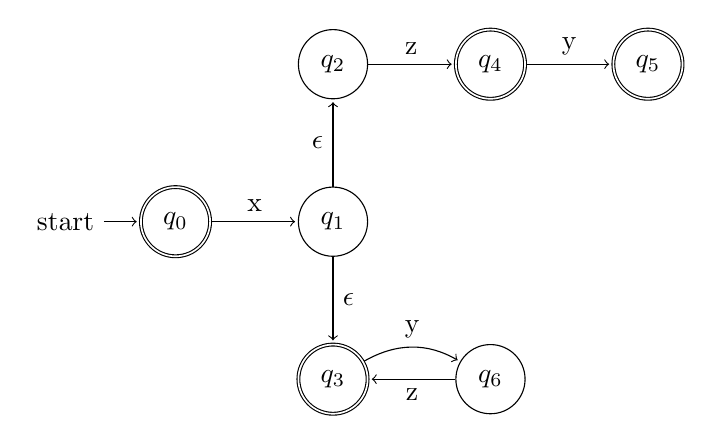
\begin{tikzpicture}[shorten >=1pt,node distance=2cm,on grid,auto]
        \node[state,initial,accepting] (q_0)   {$q_0$};
\node[state] (q_1) [ right=of q_0] {$q_1$};
        \node[state] (q_2) [ above=of q_1] {$q_2$};
        \node[state,accepting] (q_3) [ below=of q_1] {$q_3$};
        \node[state,accepting] (q_4) [ right=of q_2] {$q_4$};
        \node[state,accepting] (q_5) [ right=of q_4] {$q_5$};
        \node[state] (q_6) [ right=of q_3] {$q_6$};
        \path[->]
        (q_0)
        edge  node  [above]{x} (q_1)
        (q_1) edge  node  {$\epsilon$} (q_2)
        (q_1) edge  node  {$\epsilon$} (q_3)
        (q_2) edge  node  {z} (q_4)
        (q_4) edge  node  {y} (q_5)
        (q_6) edge  node {z} (q_3)
        (q_3) edge [bend left] node {y} (q_6);
    \end{tikzpicture}
\end{solution}

\subsubsection{$(10)*1*01*0$}
\begin{solution}
  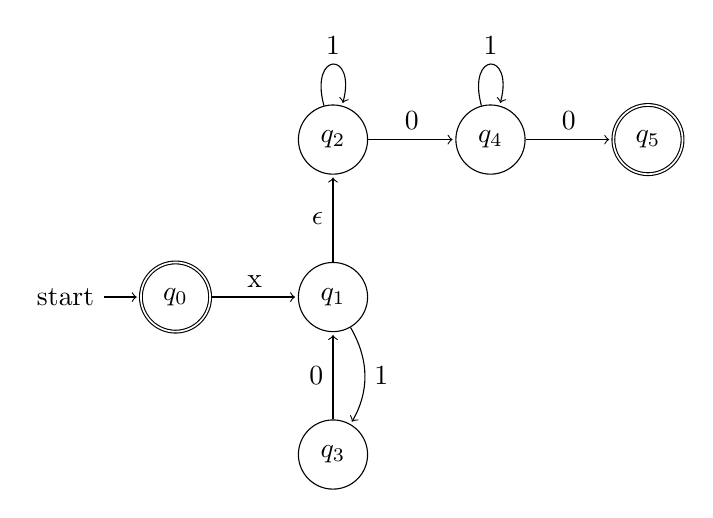
\begin{tikzpicture}[shorten >=1pt,node distance=2cm,on grid,auto]
        \node[state,initial,accepting] (q_0)   {$q_0$};
\node[state] (q_1) [ right=of q_0] {$q_1$};
        \node[state] (q_2) [ above=of q_1] {$q_2$};
        \node[state] (q_3) [ below=of q_1] {$q_3$};
        \node[state] (q_4) [ right=of q_2] {$q_4$};
        \node[state,accepting] (q_5) [ right=of q_4] {$q_5$};
        \path[->]
        (q_0)
        edge  node  [above]{x} (q_1)
        (q_1) edge  node  {$\epsilon$} (q_2)
        (q_2) edge  node  {0} (q_4)
        (q_4) edge [ loop above] node  {1} (q_4)
        (q_4) edge   node  {0} (q_5)
        (q_2) edge [ loop above] node  {1} (q_2)
        (q_3) edge  node {0} (q_1)
        (q_1) edge [bend left] node {1} (q_3);
    \end{tikzpicture}
\end{solution}
\subsubsection{Convert the NFA above to a DFA}
\begin{figure}[h]
    \centering
    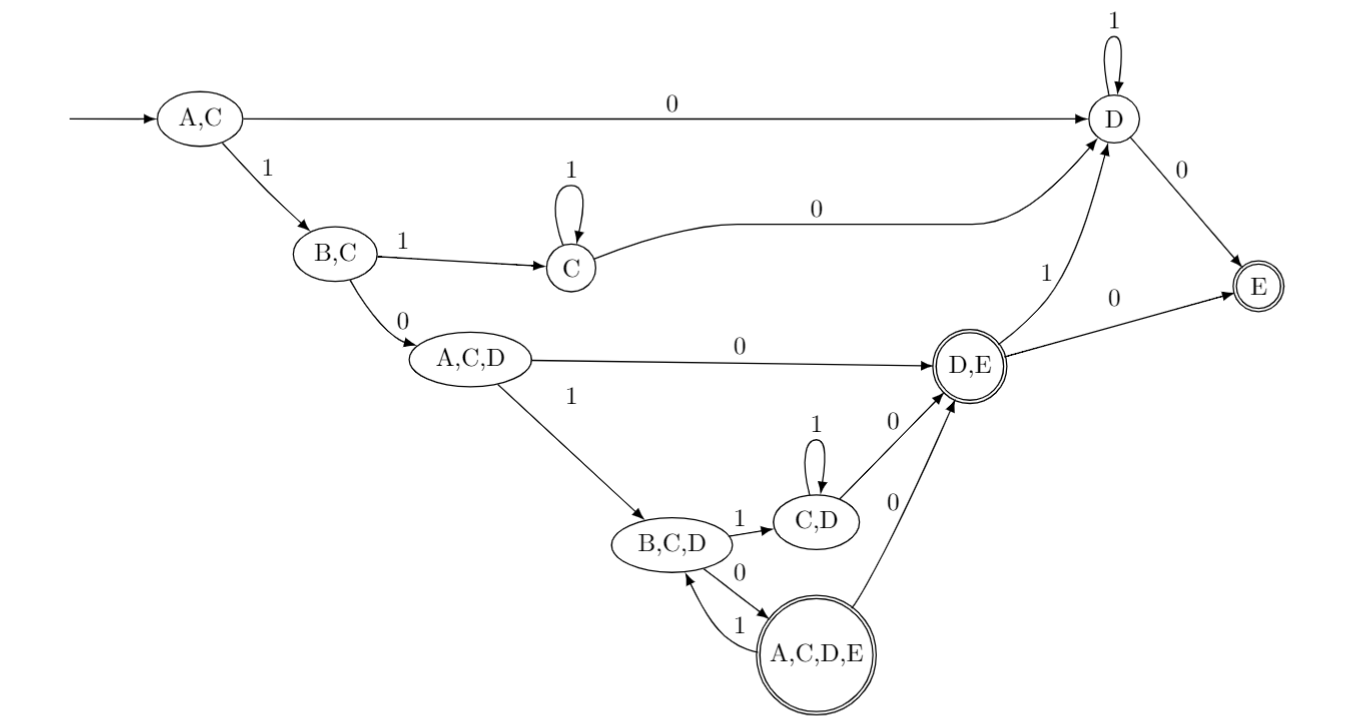
\includegraphics[width=0.7\columnwidth]{1.7.2-solution.png}
\end{figure}
\begin{solution}
\end{solution}
\subsection{Minimized the NFA}
\begin{enumerate}
    \item Original NFA, $\Sigma = \{a, b, c\}$:
          \\
          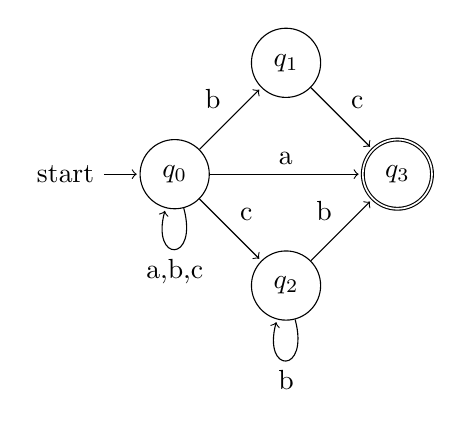
\begin{tikzpicture}[shorten >=1pt,node distance=2cm,on grid,auto]
              \node[state,initial] (q_0)   {$q_0$};
              \node[state] (q_1) [above right=of q_0] {$q_1$};
              \node[state] (q_2) [below right=of q_0] {$q_2$};
              \node[state,accepting](q_3) [below right=of q_1] {$q_3$};
              \path[->]
              (q_0) edge [loop below] node {a,b,c} ()
              edge  node  [above] {a} (q_3)
              edge  node  {b} (q_1)
              edge  node  {c} (q_2)
              (q_1) edge  node  {c} (q_3)
              (q_2) edge  node  {b} (q_3)
              edge  [loop below] node  {b} ();
          \end{tikzpicture}

\begin{solution}
 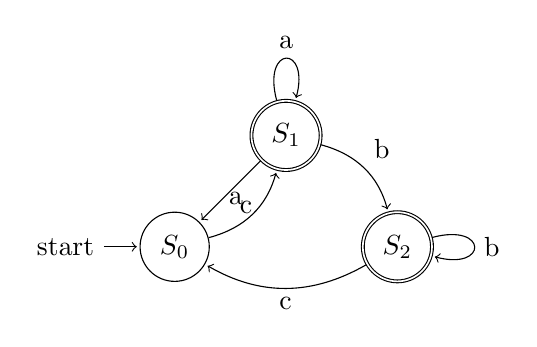
\begin{tikzpicture}[shorten >=1pt,node distance=2cm,on grid,auto]
                %% Your answer here
                \node[state,initial] (S_0)   {$S_0$};
                \node[state,accepting] (S_1) [above right=of S_0] {$S_1$};
                % \node[state] (S_3) [below right=of S_0] {$S_3$};
                \node[state,accepting](S_2) [below right=of S_1] {$S_2$};
                % \node[state,accepting](S_6) [below right=of S_4] {$S_6$};
                \path[->]
                (S_0) %edge [loop below] node {a,b,c} ()
                      edge [bend right] node  {a} (S_1)
                    %   edge  node  {b,c} (S_2)
                    %   edge  node  {c} (S_3)
                (S_1) edge [bend left] node  {b} (S_2)
                edge  node  {c} (S_0)
                edge [loop above] node {a} ()
                % (S_2) edge  node  {a} (S_2)
                % edge  node  {b,c} (S_4)
                % edge [loop above] node {b} ()
                
                (S_2) edge [bend left] node  {c} (S_0)
                % edge  node  {a} (S_4)
                edge [loop right] node {b} ();
                % (S_5)% edge  node  {a} (S_5)
                % edge  node  {b} (S_6)
                % edge [loop above] node {a,c} ();
                
                %(S_6) edge  node  {a} (S_5)
                %edge  node  {b} (\S_6)
                %edge [loop above] node {c} ()
    \end{tikzpicture}
\end{solution}
\end{enumerate}
\section{Pumping Lemma \cite{pumpinglemma}}
Pumping Lemma: For any DFA (or NFA or regular expression) that accepts an infinite number of strings, there is some minimum length, \(M,\) such that any string
with length greater than or equal to \(M\) that the machine accepts must have the form
\(u x v,\) where \(u, x,\) and \(v\) are strings, \(x\) is not empty, the length of \(u x\) is \(\leq M,\) and the
machine accepts all strings of the form \(u x^{n} v,\) for all \(n \geq 0\).
\subsection{Proof of not regular} Let \(A=\left\{1^{j} z \mid z \in\{0,1\}^{*}\right.\) and \(z\) contains at most \(j\) i's, for any \(\left.j \geq 1\right\} .\) Prove, by the
pumping lemma, that \(A\) is not regular.\\
\begin{solution}
    Let $M$ be the minimum length as in the pumping lemma, for the regular language $A$. Select $s=1^{M} 01^{M}$, which is accepted by $A$. The pumping lemma says that if $A$ is regular, there is a decomposition $s=u x v$ such that $|x|>0,|u x| \leq M$, and $u x^{n} v \in A$ for all $n \geq 0$. Since $|u x| \leq M$, the substring $u x$ must be entirely contained within the initial $1^{M}$ substring of $s$. Thus, $u=1^{p}$ and $x=1^{q}$ for some integers $p$ and $q$ such that $p \geq 0, q \geq 1,($ since $q=|x|>0)$, and $p+q \leq M$.

    Then $s=u x v=1^{p} 1^{q} 1^{M-p-q} 01^{M} .$ Now $u x^{n} v$ is supposed to be in $A$ for any $n \geq 0$, so in particular $u x^{0} v=u v$ should be in $A$.

    But $u v=1^{p} 1^{M-p-q} 01^{M}=1^{M-q} 01^{M}$, and $q \geq 1$, so $M-q<M$. This word begins with $M-q$ ones followed by a zero, so if we try to match it up with the form $1^{j} z$ in the definition of $A$, the largest value of $j$ that it can match is $j=M-q$, which is less than $M$. But then $z$ has to be $01^{M}$, which has more than $j$ ones, and thus $u v$ can't be in $A$ after all. This is a contradiction, and consequently $A$ is not regular.
\end{solution}


\section{Derivations in Top-down parsing}

If a string belongs to a particular language, we can find a parse tree for it.  A single nonterminal  roots  the  parse  tree  (e.g  ‘prog’  or  ‘expr’).   This  top-level  nonterminal branches off into constituent nonterminals, eventually breaking down into terminals and symbols at the leaves.Top-down parsing is a method of matching strings via an abstract preorder traversal of a parse tree.  We’ve already seen an example of this: recursive descent!  As a recap from lecture:
\begin {enumerate}
\item \textbf{Leftmost derivation:}  a  sequence  of  rules  following  a preorder traversal  of  the parse tree.
\item \textbf{Rightmost derivation:} see previous definition, but with a right-to-left preorder traversal.
\end{enumerate}

The reverse rightmost derivation is the rightmost derivation in reverse.  The reverse rightmost derivation is an instance of bottom-up parsing—the string’s lowest level de-tails are recognized first, then mid-level details, finally leading up to the start symbol.

\section{Lambda Expression\cite{byvoidlambda}}

\subsection{Start with halting problems}

You must have heard of "object-oriented": encapsulation, inheritance, polymorphism, all in all it seems to be very powerful. Functionality sounds like a real weakness.
\\
Functional programming is a completely different programming paradigm, as opposed to "imperative programming". It is characterized by: invariants, inertia, high order functions, no side effects, everything is a function.

Have you ever thought of a tool that automatically checks for dead loops in your program? Whether you have ever thought about it or not, I have anyway, but unfortunately the answer is, no!

\textbf{Halting problem:} Given any program and its input, determine whether the program can end within a finite number of calculations. Assuming that this algorithm is actually made, you can just give it any function and the input to this function, and it will tell you whether the function will run to the end or not.
We describe this in the following pseudo-code:


\begin{figure}[H]
    \begin{minted}[mathescape, linenos]{c}
function halting(func, input) {
    return if_func_will_halt_on_input;
}
    \end{minted}
\end{figure}
and another pseudo-code:
\begin{figure}[H]
     \begin{minted}[mathescape, linenos]{c}
function ni_ma(func) {
    if (halting(func, func)) {
        for(;;) //dead loop }
}
    \end{minted}
\end{figure}

When we call \textbf { ni\_ma(ni\_ma) }. We can't deduce whether it is halting or not halting. Thus halting problem is not deciable.


Here comes the \textbf{lambda calculus}, Consider the following \textbf{lambda calculus} grammar:
\subsection{What language is accepted by the following DFA?}
\begin{verbatim}
var  : ID ;
expr : var
     . ‘(’ ‘l’ var ‘.’ expr ‘)’
     | ‘(’ expr expr ‘)’ ;
\end{verbatim}

Use this \cite{lambdacpptest} to construct leftmost and reverse rightmost derivations of the following strings.
\\
\texttt{($\lambda$ f .($\lambda$ x .(f(f x))))}
\\
Of the three syntaxes defined earlier, the first two are used to generate \textit{functions} and the third is used for function \textit{calls}, e.g.:  \texttt{(($\lambda$ xy.x+y)23)}. For simplicity:  \texttt{let add= $\lambda$ xy.x+y then (add 2 3)}\\

Here's the two axiom of \textbf{lambda calculus}:
\begin{enumerate}
\item \textbf{Permutation axiom:} \texttt{$\lambda$ xy.x+y=> $\lambda$ ab.a+b}
\item \textbf{Substitute axiom:} \texttt{($\lambda$ xy.x+y)ab=>a+b}
\end{enumerate}

\subsection{Function Generator}

The $\lambda$ algorithm is equivalent to a function generator
\begin{enumerate}
    \item \texttt{let mul= $\lambda$ xy.x*y}, we have: \texttt{mul 3 5 -> 3 * 5}
    \item \texttt{let con= $\lambda$ xy.xy}, we have: \texttt{con ‘yangyw’ ‘ISvegetable’ -> ‘yangywISvegetable’}
    \item \texttt{let not = false -> true . true -> false}
    \item \texttt{let ext-and = true value -> value . false value -> false . value true -> value . value false -> false}
    \item \texttt{let if = $\lambda$ cond tvalue fvalue . (cond and tvalue) or (not cond and fvalue)}
    \item \texttt{let fact =$\lambda$ n . if (n==0) 1 (n * fact n-1)}
\end{enumerate}
We noticed that the sixth take the function itself as the input for the function. It's not in accordance to the math axiom loop definition and can be parsed by compilers. It will parameterize itself as $self$:
\\
\\
\texttt{let P = $\lambda$ self n . if (n==0) 1 (n * self(self n-1))}\\
\texttt{let fact n = P (P n)}
\\

Unfortunately this isn't really recursive, it's just an extra argument passed in each time and called repeatedly. So what is our purpose? I want a truly recursive function that is

\begin{solution}
$Y(P)=$ fact $=\lambda n .$ if $(n==0) 1(n *$ fact
$n-1)$
\end{solution}

\subsection{Fixed Point P(fact) = fact}
What is a fixed point? It is a point (in the generalized sense) that is mapped by a function, and the result obtained is still the point. Imagine a map of China on the wall falls on the floor, there must be and only one point on the map with its actual position.
\subsection{Magical Y}
So let's go ahead and assume that there is a magic function Y that finds the immovable point of this pseudo-recursive function, namely:

\texttt{Y(F) = f = F(Y(F)), where F(f) = f and Y(P) = fact }
Let's construct the Y Combinator (a starter helper in Silicon Valley.)
\begin{enumerate}
    \item \texttt{let Y = $\lambda$ F . G (G), where G =  $\lambda$ self. F(self(self))}
\end{enumerate}

\begin{equation}
    \begin{split}
        \texttt{Y(P)} &=\texttt{G(G)}\texttt{ where  G = }\lambda\texttt{ self. P(self(self))}\\
&= \texttt{P(G(G))}\\
&= \lambda \texttt{n. if (n==0) 1 (n * G(G) n-1)}\\
\end{split}
\end{equation}
Suppose Y(P) = fact,then Y(P) = fact = $\lambda$ n. if (n==0) 1 (n * fact n-1)

Only if we have Y, we can transform the pseudo-recursive function into the true recursive function we want. Now when we want to define a recursive function, we just add a self parameter, define it in a pseudo-recursive way, and then use the Y-combination subset to make it the true recursion we want.

\subsection{Turing Equivalence}

We have successfully derived the Y-combinator, which is equivalent to deriving a theorem in the \textbf{lambda calculus} axiomatic system:
 It is possible to refer to itself in the process of defining a function This theorem is an important step in proving the Turing equivalence of \textbf{lambda calculus}s. What does it mean that the \textbf{lambda calculus} is Turing-equivalent?

It means that its computational power is identical to that of our computers. It means that any program can be described by the \textbf{lambda calculus}, and that the functions described by the \textbf{lambda calculus} must be computable by a computer.

Recall that we just talked about the stopping problem, i.e., the undecidability of whether a Turing machine can stop when given an arbitrary input.
The equivalent of this proposition in the \textbf{lambda calculus} is: There does not exist an algorithm that can determine whether any two $\lambda$-functions are equivalent, i.e., have \texttt{f(n) = g(n)} for all \texttt{n}.

\subsection{Functional Programming}

Haskell is a purely functional programming language, named in honor of Haskell Curry. Everything in Haskell is a function, not even the concept of variables in imperative programming; all its variables are allowed to be assigned only once and then are immutable, just like the assignment of variables in mathematical derivation.

Haskell also does not have a control flow structure in the usual sense, such as for loops, but instead has recursion. two other important features of Haskell are side-effect free and inertial evaluation. No side effects means that any function given the same input will have the same result every time it is called, and inertial evaluation means that the function will not compute immediately unless needed. Here's Some examples in Haskell:

Before running the Haskell program, first you need to install a \texttt{GHC} compiler, and then run \texttt{ghci} to enter interactive mode. Here are some example
\begin{enumerate}
    \item \texttt{let max a b = if a>b then a else b}
    \begin{enumerate}
        \item \texttt{max 3 4 = 4}
        \item \texttt{max 1.0001 1 = 1.0001}
        \item \texttt{max "victoryang00" "CmYkRgB123" = "CmYkRgB123"}
    \end{enumerate}
    \item \textbf{List Annotation:}
    
    \texttt{list X ::= [] | elem: (list  X)}
    \begin{enumerate}
        \item \texttt{[ 1 ] = 1:[]}
        \item \texttt{[ 1,2,3 ] = 1:2:3:[]}
        \item \texttt{[ 1,3 .. ] = [1,3,5,...]}
    \end{enumerate}
    \item \textbf{Pattern Recognition:} \texttt{let first (elem:rest) = elem}
    \begin{enumerate}
        \item \texttt{first [1,3] = 1, pairing (1,3:[])}
    \end{enumerate}
    \item \textbf{List Sum:} \texttt{accumulate (elem:rest) = elem + accumulate rest}
    \item \textbf{Palindrome:} 
    
    \texttt{palindrome []  = True}
    
     \texttt{palindrome [\_] = True}
     
     \texttt{palindrome (elem:rest) = (elem == last rest) \&\& (palindrome(init rest))}
     \item \textbf{Lazy Evaluation:} \texttt{[1,3..] !! 42 = 85}
     \item \textbf{Linear Fibbonacci:} \texttt{fib = 1:1:zipWith (+) fib (tail fib)}
\end{enumerate}

\section{Recursive Descent Parsers}
It is a kind of Top-Down Parser. A top-down parser builds the parse tree from the top to down, starting with the start non-terminal. A Predictive Parser is a special case of Recursive Descent Parser, where no Back Tracking is required.
By carefully writing a grammar means eliminating left recursion and left factoring from it, the resulting grammar will be a grammar that can be parsed by a recursive descent parser.


Try writing a recursive descent parser for \textbf{lambda calculus}.  Assume the existence of $LITERAL(C)$, $yynext()$, and $yyerror()$ in flex.

\begin{solution}
\begin{alltt}
def var():
    if yynext() == IDENT:
        return Var(yyscan(yynext()))
    else:
        yyerror()
def expr():
    if yynext()== '(':
        return var()
    yyscan('(')
    if yynext()== '\(\lambad\)':
        yyscan('\(\lambda\)')
        param = var()
        yyscan('.')
        body = expr()
        yyscan('(')
        return new Lambda(param, body)
    else:
        func = expr()
        args = expr()
        yyscan(')')
        return FunCall(func, args)
\end{alltt}
\end{solution}
\subsection{Ambiguous Grammars}
A grammar is ambiguous if it permits multiple distinct parse trees for some string.For example, without the order of operations, \texttt{12−8/4} could parse as 1 or as 10.  Make the following grammar unambiguous, and also give precedence to ‘/’ over ‘-’.

\begin{verbatim}
e : INT
  | e ‘-’ e
  | e ‘/’ e 
\end{verbatim}

\subsubsection{Eliminate the left factoring}

As another example is called dangling else, consider the following grammar:

\begin{verbatim}
expr,stmt,other : 0 | 1 

stmt : other
     | if expr then stmt
     | if expr then stmt else stmt
\end{verbatim}
When seeing the input notation if, one cannot immediately determine which generator to use to extend $s t m t$.
In general, if $A \rightarrow \alpha \beta_{1} \mid \alpha \beta_{2}$ is two generators of $A$, and the prefix of the input string is a non-empty string derived from $\alpha$, after looking at the input from $\alpha$, then extend $A^{\prime}$ to $\alpha_{1}$ or $\beta_{2}$. $beta_{1}$ or $\beta_{2}$. This is the left lifting factor, and the original generating equation becomes:
$$A \rightarrow \alpha A^{\prime}$$
$$A^{\prime} \rightarrow \beta_{1} \mid \beta_{2}$$

Left factoring the above grammar.

\begin{solution}
$$\text{stmt} \longrightarrow \text{\textbb{if} expr \textbb{then} stmt optional\_else\_part} \\ \mid \text{\textbb{other}}$$
$$\text{optional\_else\_part} \rightarrow \text{\textbb{else} stmt} \mid \epsilon$$
\end{solution}

Give an example of a string in the language that can produce multiple parse trees.

\begin{solution}
\begin{verbatim}
if 0 then if 1 then $0 ;$ else 1 ;
\end{verbatim}
The two parse trees corresponding to this statement could be:
\begin{enumerate}
    \item \begin{verbatim}
if 0 then (if 1 then 0 ; else $1 ;$ )
\end{verbatim}
\item \begin{verbatim}
if 0 then (if 1 then 0 ; ) else 1 ;
\end{verbatim}
\end{enumerate}
\end{solution}
How to resolve the problem?

\begin{solution}

\end{solution}

\subsubsection{Eliminate the left recursion}
A grammar is left-recursive if it has a non-terminator $A$, and for some string $\alpha$, there exists a derivation $A \Rightarrow{ }^{+} A \alpha$. The top-down analysis method cannot be used for left-recursive grammars, so it is necessary to eliminate left recursion. The left recursion induced by generators of the form $A \rightarrow A \alpha$ is called direct left recursion.

The left recursive generating equation $A \rightarrow A \alpha \mid \beta$ can be used in a non-left recursive

$$A \rightarrow \beta A^{\prime}$$
$$A^{\prime} \rightarrow \alpha\left|A^{\prime}\right| \varepsilon$$

Generally from $A \rightarrow A \alpha_{1}\left|A \alpha_{2}\right| \cdots\left|A \alpha_{m}\right| \beta_{1}\left|\beta_{2}\right| \cdots \mid \beta_{n}$ to 

$$A \rightarrow \beta_{1} A^{\prime}\left|\beta_{2} A^{\prime}\right| \cdots \mid \beta_{n} A^{\prime}$$
$$A^{\prime} \rightarrow \alpha_{1} A^{\prime}\left|\alpha_{2} A^{\prime}\right| \cdots\left|\alpha_{m} A^{\prime}\right| \varepsilon$$Use this grammar to construct leftmost and reverse rightmost derivations of the following strings.
\begin{enumerate}
\item \textbb{Consider the example and eliminate the direct left recursion}

$$E \rightarrow E+T \mid T$$
$$T \rightarrow T * F \mid F$$
$$F \rightarrow(E) \mid\text{ id}$$ 

\begin{solution}
$$E \rightarrow T E^{\prime}$$
$$E^{\prime} \rightarrow+T E^{\prime} \mid \varepsilon$$
$$T \rightarrow F T^{\prime}$$
$$T^{\prime} \rightarrow * T^{\prime} \mid \varepsilon$$
$$F \rightarrow(E) \mid$$ id
\end{solution}
\item \textbb{Consider the example and eliminate the indirect left recursion}
$S \rightarrow A a \mid b$
$A \rightarrow S d \mid \varepsilon$
\end{enumerate}


\subsection{Syntax-directed Translation}
Parser-generators usually support syntax-directed translation, which is a convenient way  to  execute  an  action  every  time  a  grammar  rule  is  matched.   While  defining actions,  the  variable \$\$ refers  to  a  location  into  which  the  semantic  value  of  the current symbol can be stored.  The variables \$1, ...,\$n refer to the semantic values of the symbols used to match the current rule.  Here’s an example:
\begin{verbatim}
p : e ’;’        { printf("Result: %d\n", $1); }

e : INT          { $$ = $1; }
  | e ‘-’ e      { $$ = $1 - $3; }
  | e ‘/’ e      { $$ = $1 / $3; } ;
\end{verbatim}

Write a syntax-directed translator for the first grammar you wrote for this \textbf{Simple Caculator}.

\begin{solution}
\begin{verbatim}
em : INT       { $$=$1 ;}
   | em '/' em { $$=$1 / $3;} ;
e  : em        { $$=$1 ;}
   | e '-' e   { $$=$1 - $3;} ;
\end{verbatim}
\end{solution}
Write for \textbf{lambda calculus}.

\begin{solution}
\begin{alltt}
var   : ID         { $$=new var($1) ;}
expr  : var        { $$=$1 ;}
      | '(' '\(\lambda\)' var '.' expr ')'   { $$=new lambda($3, $5);} 
      | '(' expr expr ')'   { $$=new funcall($2, $3);} ;
\end{alltt}
\end{solution}

\printbibliography
\end{document}
